\documentclass{standalone}
\usepackage{tikz}
\usetikzlibrary{patterns, positioning}


\begin{document}
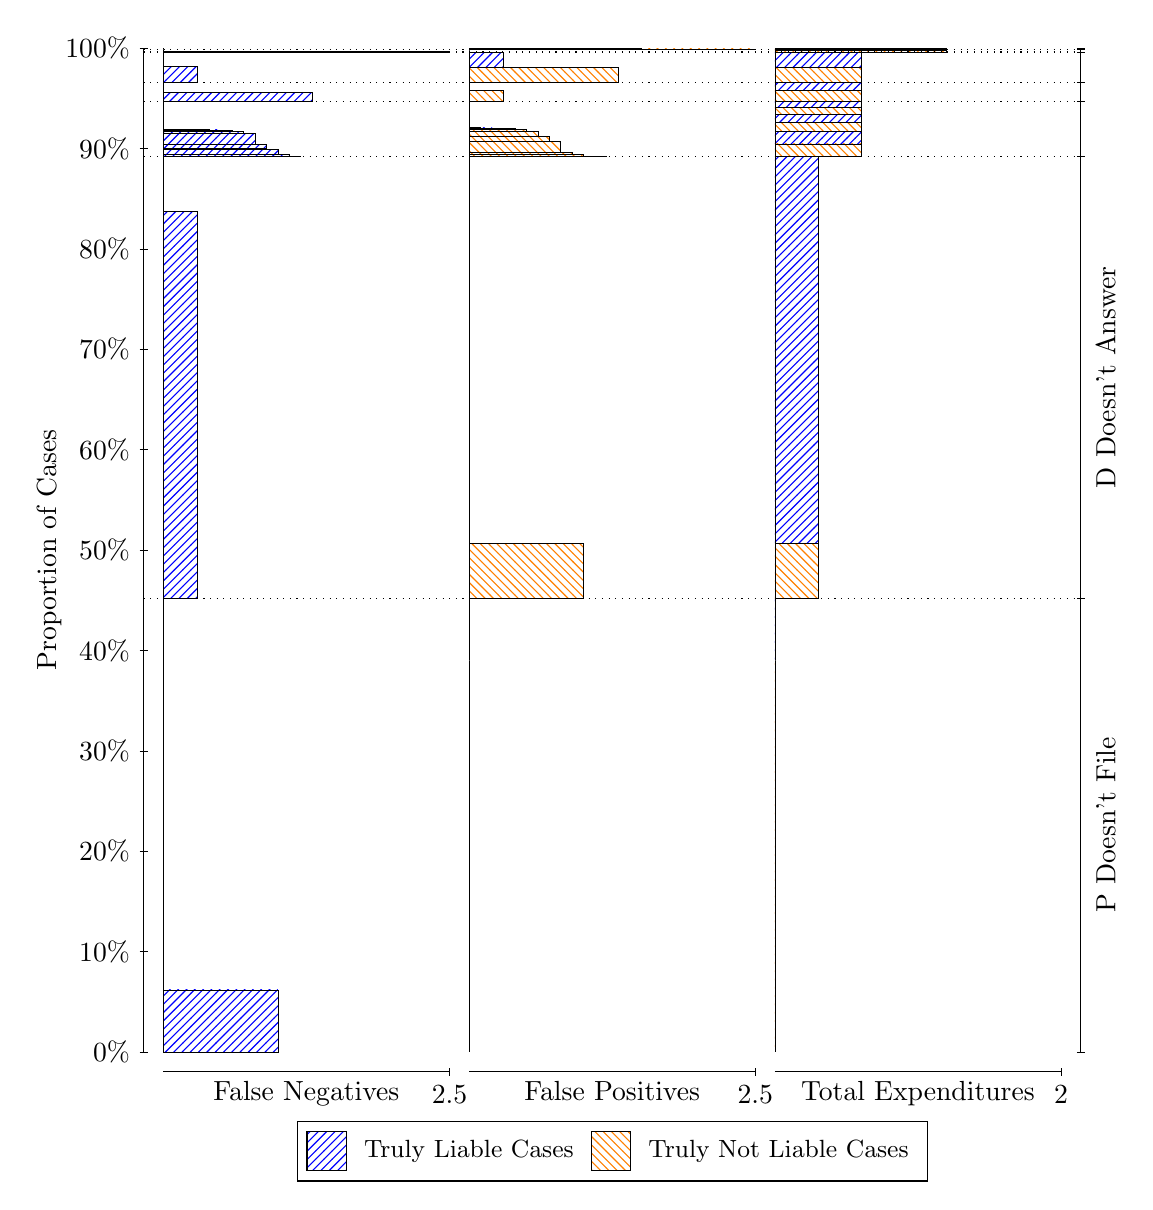
\begin{tikzpicture}
\draw[black, very thin] (1.5,1.75) -- (1.5,14.5);
\node[rotate=90, text=black, anchor=center] at (0.3, 8.125) {Proportion of Cases};
\draw[black, very thin] (1.45,1.75) -- (1.55,1.75);
\node[text=black, anchor=east] at (1.45, 1.75) {0\%};
\draw[black, very thin] (1.45,3.025) -- (1.55,3.025);
\node[text=black, anchor=east] at (1.45, 3.025) {10\%};
\draw[black, very thin] (1.45,4.3) -- (1.55,4.3);
\node[text=black, anchor=east] at (1.45, 4.3) {20\%};
\draw[black, very thin] (1.45,5.575) -- (1.55,5.575);
\node[text=black, anchor=east] at (1.45, 5.575) {30\%};
\draw[black, very thin] (1.45,6.85) -- (1.55,6.85);
\node[text=black, anchor=east] at (1.45, 6.85) {40\%};
\draw[black, very thin] (1.45,8.125) -- (1.55,8.125);
\node[text=black, anchor=east] at (1.45, 8.125) {50\%};
\draw[black, very thin] (1.45,9.4) -- (1.55,9.4);
\node[text=black, anchor=east] at (1.45, 9.4) {60\%};
\draw[black, very thin] (1.45,10.675) -- (1.55,10.675);
\node[text=black, anchor=east] at (1.45, 10.675) {70\%};
\draw[black, very thin] (1.45,11.95) -- (1.55,11.95);
\node[text=black, anchor=east] at (1.45, 11.95) {80\%};
\draw[black, very thin] (1.45,13.225) -- (1.55,13.225);
\node[text=black, anchor=east] at (1.45, 13.225) {90\%};
\draw[black, very thin] (1.45,14.5) -- (1.55,14.5);
\node[text=black, anchor=east] at (1.45, 14.5) {100\%};

\draw[black, very thin] (13.4,1.75) -- (13.4,14.5);
\draw[black, very thin] (13.35,1.75) -- (13.45,1.75);
\node[anchor=west] at (13.35, 1.75) {};
\draw[black, very thin] (13.35,7.5137) -- (13.45,7.5137);
\node[anchor=west] at (13.35, 7.5137) {};
\draw[black, very thin] (13.35,13.12) -- (13.45,13.12);
\node[anchor=west] at (13.35, 13.12) {};
\draw[black, very thin] (13.35,13.826) -- (13.45,13.826);
\node[anchor=west] at (13.35, 13.826) {};
\draw[black, very thin] (13.35,14.066) -- (13.45,14.066);
\node[anchor=west] at (13.35, 14.066) {};
\draw[black, very thin] (13.35,14.449) -- (13.45,14.449);
\node[anchor=west] at (13.35, 14.449) {};
\draw[black, very thin] (13.35,14.482) -- (13.45,14.482);
\node[anchor=west] at (13.35, 14.482) {};
\draw[black, very thin] (13.35,14.5) -- (13.45,14.5);
\node[anchor=west] at (13.35, 14.5) {};

\draw[black, very thin, pattern color=blue, pattern=north east lines] (1.75,1.75) rectangle (3.2033,2.5394);
\draw[black, very thin, pattern color=orange, pattern=north west lines] (1.75,2.5394) rectangle (1.75,7.5137);
\draw[black, very thin, pattern color=blue, pattern=north east lines] (1.75,7.5137) rectangle (2.186,12.426);
\draw[black, very thin, pattern color=orange, pattern=north west lines] (1.75,12.426) rectangle (1.75,13.12);
\draw[black, very thin, pattern color=blue, pattern=north east lines] (1.75,13.12) rectangle (3.494,13.126);
\draw[black, very thin, pattern color=blue, pattern=north east lines] (1.75,13.126) rectangle (3.3487,13.148);
\draw[black, very thin, pattern color=blue, pattern=north east lines] (1.75,13.148) rectangle (3.2033,13.217);
\draw[black, very thin, pattern color=blue, pattern=north east lines] (1.75,13.217) rectangle (3.058,13.222);
\draw[black, very thin, pattern color=blue, pattern=north east lines] (1.75,13.222) rectangle (3.058,13.276);
\draw[black, very thin, pattern color=blue, pattern=north east lines] (1.75,13.276) rectangle (2.9127,13.413);
\draw[black, very thin, pattern color=blue, pattern=north east lines] (1.75,13.413) rectangle (2.7673,13.439);
\draw[black, very thin, pattern color=blue, pattern=north east lines] (1.75,13.439) rectangle (2.622,13.457);
\draw[black, very thin, pattern color=blue, pattern=north east lines] (1.75,13.457) rectangle (2.4767,13.461);
\draw[black, very thin, pattern color=blue, pattern=north east lines] (1.75,13.461) rectangle (2.3313,13.465);
\draw[black, very thin, pattern color=orange, pattern=north west lines] (1.75,13.465) rectangle (1.75,13.826);
\draw[black, very thin, pattern color=blue, pattern=north east lines] (1.75,13.826) rectangle (3.6393,13.935);
\draw[black, very thin, pattern color=orange, pattern=north west lines] (1.75,13.935) rectangle (1.75,14.066);
\draw[black, very thin, pattern color=blue, pattern=north east lines] (1.75,14.066) rectangle (2.186,14.265);
\draw[black, very thin, pattern color=orange, pattern=north west lines] (1.75,14.265) rectangle (1.75,14.449);
\draw[black, very thin, pattern color=blue, pattern=north east lines] (1.75,14.449) rectangle (5.3833,14.46);
\draw[black, very thin, pattern color=orange, pattern=north west lines] (1.75,14.46) rectangle (1.75,14.482);
\draw[black, very thin, pattern color=orange, pattern=north west lines] (1.75,14.482) rectangle (1.75,14.49);
\draw[black, very thin, pattern color=blue, pattern=north east lines] (1.75,14.49) rectangle (1.75,14.5);
\draw[black, very thin, pattern color=orange, pattern=north west lines] (5.6333,1.75) rectangle (5.6333,6.7243);
\draw[black, very thin, pattern color=blue, pattern=north east lines] (5.6333,6.7243) rectangle (5.6333,7.5137);
\draw[black, very thin, pattern color=orange, pattern=north west lines] (5.6333,7.5137) rectangle (7.0867,8.208);
\draw[black, very thin, pattern color=blue, pattern=north east lines] (5.6333,8.208) rectangle (5.6333,13.12);
\draw[black, very thin, pattern color=orange, pattern=north west lines] (5.6333,13.12) rectangle (7.3773,13.125);
\draw[black, very thin, pattern color=orange, pattern=north west lines] (5.6333,13.125) rectangle (7.232,13.128);
\draw[black, very thin, pattern color=orange, pattern=north west lines] (5.6333,13.128) rectangle (7.0867,13.147);
\draw[black, very thin, pattern color=orange, pattern=north west lines] (5.6333,13.147) rectangle (6.9413,13.175);
\draw[black, very thin, pattern color=orange, pattern=north west lines] (5.6333,13.175) rectangle (6.796,13.314);
\draw[black, very thin, pattern color=orange, pattern=north west lines] (5.6333,13.314) rectangle (6.6507,13.373);
\draw[black, very thin, pattern color=orange, pattern=north west lines] (5.6333,13.373) rectangle (6.5053,13.446);
\draw[black, very thin, pattern color=orange, pattern=north west lines] (5.6333,13.446) rectangle (6.36,13.47);
\draw[black, very thin, pattern color=orange, pattern=north west lines] (5.6333,13.47) rectangle (6.2147,13.481);
\draw[black, very thin, pattern color=blue, pattern=north east lines] (5.6333,13.481) rectangle (5.924,13.485);
\draw[black, very thin, pattern color=blue, pattern=north east lines] (5.6333,13.485) rectangle (5.7787,13.489);
\draw[black, very thin, pattern color=blue, pattern=north east lines] (5.6333,13.489) rectangle (5.6333,13.826);
\draw[black, very thin, pattern color=orange, pattern=north west lines] (5.6333,13.826) rectangle (6.0693,13.958);
\draw[black, very thin, pattern color=blue, pattern=north east lines] (5.6333,13.958) rectangle (5.6333,14.066);
\draw[black, very thin, pattern color=orange, pattern=north west lines] (5.6333,14.066) rectangle (7.5227,14.25);
\draw[black, very thin, pattern color=blue, pattern=north east lines] (5.6333,14.25) rectangle (6.0693,14.449);
\draw[black, very thin, pattern color=orange, pattern=north west lines] (5.6333,14.449) rectangle (5.6333,14.471);
\draw[black, very thin, pattern color=blue, pattern=north east lines] (5.6333,14.471) rectangle (5.6333,14.482);
\draw[black, very thin, pattern color=orange, pattern=north west lines] (5.6333,14.482) rectangle (9.2667,14.49);
\draw[black, very thin, pattern color=blue, pattern=north east lines] (5.6333,14.49) rectangle (7.8133,14.5);
\draw[black, very thin, pattern color=orange, pattern=north west lines] (9.5167,1.75) rectangle (9.5167,6.7243);
\draw[black, very thin, pattern color=blue, pattern=north east lines] (9.5167,6.7243) rectangle (9.5167,7.5137);
\draw[black, very thin, pattern color=orange, pattern=north west lines] (9.5167,7.5137) rectangle (10.062,8.208);
\draw[black, very thin, pattern color=blue, pattern=north east lines] (9.5167,8.208) rectangle (10.062,13.12);
\draw[black, very thin, pattern color=orange, pattern=north west lines] (9.5167,13.12) rectangle (10.607,13.282);
\draw[black, very thin, pattern color=blue, pattern=north east lines] (9.5167,13.282) rectangle (10.607,13.441);
\draw[black, very thin, pattern color=orange, pattern=north west lines] (9.5167,13.441) rectangle (10.607,13.553);
\draw[black, very thin, pattern color=blue, pattern=north east lines] (9.5167,13.553) rectangle (10.607,13.655);
\draw[black, very thin, pattern color=orange, pattern=north west lines] (9.5167,13.655) rectangle (10.607,13.742);
\draw[black, very thin, pattern color=blue, pattern=north east lines] (9.5167,13.742) rectangle (10.607,13.826);
\draw[black, very thin, pattern color=orange, pattern=north west lines] (9.5167,13.826) rectangle (10.607,13.958);
\draw[black, very thin, pattern color=blue, pattern=north east lines] (9.5167,13.958) rectangle (10.607,14.066);
\draw[black, very thin, pattern color=orange, pattern=north west lines] (9.5167,14.066) rectangle (10.607,14.25);
\draw[black, very thin, pattern color=blue, pattern=north east lines] (9.5167,14.25) rectangle (10.607,14.449);
\draw[black, very thin, pattern color=orange, pattern=north west lines] (9.5167,14.449) rectangle (11.697,14.471);
\draw[black, very thin, pattern color=blue, pattern=north east lines] (9.5167,14.471) rectangle (11.697,14.482);
\draw[black, very thin, pattern color=orange, pattern=north west lines] (9.5167,14.482) rectangle (11.697,14.49);
\draw[black, very thin, pattern color=blue, pattern=north east lines] (9.5167,14.49) rectangle (11.697,14.5);
\draw[black, dotted] (1.5,7.5137) -- (13.4,7.5137);
\draw[black, dotted] (1.5,13.12) -- (13.4,13.12);
\draw[black, dotted] (1.5,13.826) -- (13.4,13.826);
\draw[black, dotted] (1.5,14.066) -- (13.4,14.066);
\draw[black, dotted] (1.5,14.449) -- (13.4,14.449);
\draw[black, dotted] (1.5,14.482) -- (13.4,14.482);
\draw[black, very thin] (1.75,1.5) -- (5.3833,1.5);
\node[text=black, anchor=north] at (3.5667, 1.5) {False Negatives};
\draw[black, very thin] (5.3833,1.45) -- (5.3833,1.55);
\node[text=black, anchor=north] at (5.3833, 1.45) {2.5};

\draw[black, very thin] (5.6333,1.5) -- (9.2667,1.5);
\node[text=black, anchor=north] at (7.45, 1.5) {False Positives};
\draw[black, very thin] (9.2667,1.45) -- (9.2667,1.55);
\node[text=black, anchor=north] at (9.2667, 1.45) {2.5};

\draw[black, very thin] (9.5167,1.5) -- (13.15,1.5);
\node[text=black, anchor=north] at (11.333, 1.5) {Total Expenditures};
\draw[black, very thin] (13.15,1.45) -- (13.15,1.55);
\node[text=black, anchor=north] at (13.15, 1.45) {2};

\node[text=black, centered, rotate=90] at (13.72, 4.6318) {P Doesn't File};
\node[text=black, centered, rotate=90] at (13.72, 10.317) {D Doesn't Answer};






\draw (7.449999999999999,1.5) node[draw=none] (baseCoordinate) {};
\begin{scope}[align=center]
        \matrix[scale=0.5, draw=black, below=0.5cm of baseCoordinate, nodes={draw}, column sep=0.1cm]{
            \node[rectangle, draw, minimum width=0.5cm, minimum height=0.5cm, pattern color=blue, pattern=north east lines] {}; &
            \node[draw=none, font=\small, text=black] (B) {Truly Liable Cases}; &
            \node[rectangle, draw, minimum width=0.5cm, minimum height=0.5cm, pattern color=orange, pattern=north west lines] {}; &
            \node[draw=none, font=\small, text=black] (B) {Truly Not Liable Cases}; \\
            };
\end{scope}

\end{tikzpicture}
\end{document}